\chapter{Case Studies}

%short introduction
%one section for each one of the case studies
%general structure for each one of the sections
    %1) Description of the model with Event-B code
    %2) Results of the simulation

The purpose of these case studies is to test the correct integration of the encoder with the MultiVeStA tool. In total there are 3 case studies: two probabilistic programs using dices and coins, a bounded re-transmission protocol, and a program that simulates a modal operator in positive negative logic. The repository that contains the code of this integration can be found in the following repository: \url{https://github.com/dfosorio/EventB2Maude-MultiVeStA}. Furthermore, this repository contains the code of the probabilistic Event-B models, their translated versions in PMaude, and the results of the simulations. A short guide on how to use the software can also be found in this repository, for any reader that might want to test or use the tool.



\section{Dice Programs}
The dice programs, based on the Knuth \& Yao paper \cite{knuth}, were originally discovered in the PRISM model checker web page \cite{PRISMDICE}. The idea is then to translate the model from the PRISM language to probabilistic Event-B, and afterwards translate the probabilistic Event-B model into PMaude using the encoder. The resulting PMaude specification will then be verified using MultiVeStA. If the results from the MultiVeStA simulations are the same as the PRISM model checker, then we can assume that the encoding and verification process were performed correctly. The probabilistic model for the first dice program is the following:
\begin{figure}[H]
    \centering
    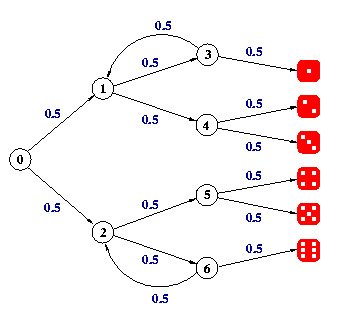
\includegraphics[scale = 0.5]{images/CS1.png}
    \caption{States and transitions of the dice model, taken from \cite{PRISMDICE}}
    \label{fig:ce1}
\end{figure}
Having as a reference the Figure \ref{fig:ce1}, the starting state of the model is the state 0. A fair coin is tossed to decide the next transition to execute. If the coin lands on heads, then the upper branch is taken. Conversely, when the coin lands on tails, the lower branch is taken. This process is repeated in each on of the sates 1 to 6, until reaching a terminating state, i.e. reaching a state where one of the dice faces is chosen. To represent this model in probabilistic Event-B, the process is straight forward: to represent all the states of the model a deferred set with all is created in the context.
\begin{maude}

CONTEXT ctxDiceProgram1
SETS 
    STATES : { s0, s1, s2, s3, s4, s5, s6, s7 }
CONSTANTS 
END
\end{maude}
where the state $s_7$ represents all the possible terminating states. In the machine of the model, two variables will be considered: one that stores the current state of the system and other that contains the current value of the dice.
\begin{maude}

MACHINE DiceProgram1
  SEES ctxDiceProgram1
  
  VARIABLES
    st 
    dice 
  INVARIANTS
    st : STATES
    dice : Nat 
\end{maude}
Each one of the transitions or coin tosses is represented with an event. For example, the first two transitions that start in state 0 can be represented with the event:
\begin{maude}

EVENT State0Trans 
WEIGHT 1
WHERE 
    st = s0
THEN
    st := {s1 @ 0.5 , s2 @ 0.5 }
END
\end{maude}
As seen in the event, the fifty-fifty probability of the coin toss is represented with a probabilistic assignment. For transitions that precede a terminating state, they are represented by changing the state to $s_7$, and assigning to the dice the respective value. For example, the transitions that branch out of the fourth state are represented in Event-B as:
\begin{maude}

EVENT State4Trans 
WEIGHT 1
WHERE 
    st = s4
THEN
    st := s7
    dice := {2 @ 0.5 , 3 @ 0.5 }
END    
\end{maude}
Finally, to initilize the system the values $s_0$ and 0 are assigned to the variables $st$ and $dice$ respectively.
\begin{maude}

INITIALISATION
    st := s0
    dice := 0
\end{maude}


The property that wants to be verified for this program is the probability of reaching a terminating state where the value of $dice = k$, where $k = 1,2,...,6$. if the model is correct, then the probability is $P(dice = k) = \frac{1}{6}$ for all $k$.

Using the encoder, the PMaude specification is obtained by repeating the process in Chapter 3. The file that contains this specification can be found in the repository with the filename \texttt{DiceProgram1.maude}. In order to define the user observations \texttt{rval}, an equation needs to be added that obtains the value of the dice variable. Therefore, for each one of the possible values of the dice (1 to 6) an equation is added that returns true (represented as 1.0 since \texttt{rval} return float numbers) if the dice has that specific value. For example, to verify that the dice has the value 1, the following equation is added to the PMaude specification:
\begin{maude}

  --- User Defined Observations 
eq val("obs1",{Conf < MNAME:Machine | 
                    variables:('st |-> st , 'dice |-> dice) >} 
                    {gt | SL}) 
                    = toFloat(((dice) =b (val(elt(1))))) .
\end{maude}
Hence, when the \texttt{s.rval("obs1")} is called in the MultiQuaTEx file, it will return 1.0 if the value of the dice is 1, and 0.0 otherwise. Moreover, for every encoded model, the encoder will also generate inside the specification 2 equations that can be used to define \texttt{rval} observations, regarding the terminating state of the model:
\begin{maude}

eq val("isMax", {Conf} {gt | SL}) = if (gt >= MAX-STEPS) 
                                    then 1.0 
                                    else 0.0 fi .

 eq val("deadlock", {Conf < events : Events | state: (LEv) >} 
                    {gt | SL}) = if (not-unknown(LEv) and not(one-firable(LEv))) 
                                 then 1.0 
                                 else 0.0 fi .
\end{maude}
The first equation returns 1.0 (true) if the maximum number of transitions have been exeuted. Each transition corresponds to the execution of the $chooseEvt$ rule, and the number that defines the maximum number of transitions is specified as a constant named as \texttt{MAX-STEPS} in the specification. By default it is set to 10000, but it can be modified directly in the PMaude specification. Inside the specification, this number is used to bound the number of transitions of the PMaude model, and terminating its execution when the number is reached.

The second equation returns 1.0 if the model has reached a deadlock, i.e. none of the guards of the translated events have been satisfied. To do this, the equation \texttt{not-unknown} (it verifies that all the states have a state different from \texttt{unknown}) and \texttt{one-firable} (it verifies if there is at least one event with satisfied guards) are used. It is important to understand correctly these two equations, since they will be used to define the terminating condition of most of the PMaude specifications that result from the translation. 

For the verification of the model, the MultiQuaTEx formula that is used to verify the model is:
\begin{maude2}

PDice1(n) = if ((s.rval("isMax") == 1.0) || (s.rval("deadlock") == 1.0)) 
            then s.rval(n) else # PDice1(n) fi ;

eval E[ PDice1("obs1") ] ;
eval E[ PDice1("obs2") ] ;
eval E[ PDice1("obs3") ] ;
eval E[ PDice1("obs4") ] ;
eval E[ PDice1("obs5") ] ;
eval E[ PDice1("obs6") ] ;
\end{maude2}
When a terminating state is reached, i.e. the simulation reached the maximum number of transitions or the simulation got in a deadlock state, then the formula returns the the value of the observation \texttt{s.rval(n)} where \texttt{n} is a parameter of the formula, that is going to be replaced in each one of the evaluation calls with \texttt{"obs1"},\texttt{"obs2"}... or \texttt{"obs6"}. Using this formula, and the parameters $\alpha = 0.01, \delta = 0.01$ and $bs = 28$, the results of the simulation using MultiVeStA where:
\begin{table}[H]
\centering
\begin{tabular}{|l|l|l|l|}
\hline
Property     & ObtainedValue     & Variance          & CI                  \\ \hline
PDice1(obs1) & 0.169194084235345 & 0.140571212336999 & 0.00999772484533201 \\ \hline
PDice1(obs2) & 0.165127336320909 & 0.137864066309953 & 0.00999898248710578 \\ \hline
PDice1(obs3) & 0.166322650733297 & 0.138663192561158 & 0.00999737034957979 \\ \hline
PDice1(obs4) & 0.164898271712973 & 0.137710597576251 & 0.00999724079076279 \\ \hline
PDice1(obs5) & 0.166095890410959 & 0.138511810325858 & 0.00999571303811207 \\ \hline
PDice1(obs6) & 0.167870619946092 & 0.139693840237627 & 0.00999651791545913 \\ \hline
\end{tabular}
\end{table}

\begin{figure}[H]
    \centering
    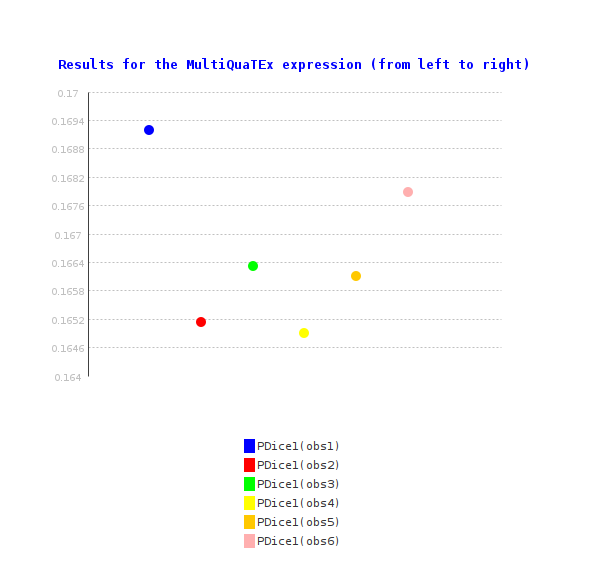
\includegraphics[scale = 0.5]{images/CS2.png}
    \caption{Graph of the simulation results of the first dice program}
    \label{fig:ce2}
\end{figure}
The total time it took to run the complete simulation was 2521.757 seconds (42 minutes). From this simulation, it is safe to say that the obtained results are close to the expected real value of $\frac{1}{6}$, and the verification of the first dice program is concluded.

The second dice program corresponds to the same scenario, but considering two dice throws, i.e. the same transition system but simulated twice. This time, the property that wants to be verified is the probability of obtaining $k$ as the sum of the results of both dice, where $k = 2,3,4,...,12$. The expected probability for each one of the possible sums of two dice is:

\begin{table}[H]
\centering
\begin{tabular}{|l|l|l}
\cline{1-2}
k  & Probability &  \\ \cline{1-2}
2  & 1/36        &  \\ \cline{1-2}
3  & 1/18        &  \\ \cline{1-2}
4  & 3/36        &  \\ \cline{1-2}
5  & 1/9         &  \\ \cline{1-2}
6  & 5/36        &  \\ \cline{1-2}
7  & 1/6         &  \\ \cline{1-2}
8  & 5/36        &  \\ \cline{1-2}
9  & 1/9         &  \\ \cline{1-2}
10 & 3/36        &  \\ \cline{1-2}
11 & 1/18        &  \\ \cline{1-2}
12 & 1/36        &  \\ \cline{1-2}
\end{tabular}
\end{table}
To specify the model, one approach would be to add new variables \textit{state2}, \textit{dice2}, and duplicate the events specified in the previous dice program to change the new variables. Event though implementing the Event-B model in this way would work, for this model the optimized version proposed in \cite{knuth} will be used. This version consists of the same principle: multiple states and coin tosses as transitions, until reaching a terminating state, i.e. the sum of two dices. The graph that represents this model is:
\begin{figure}[H]
    \centering
    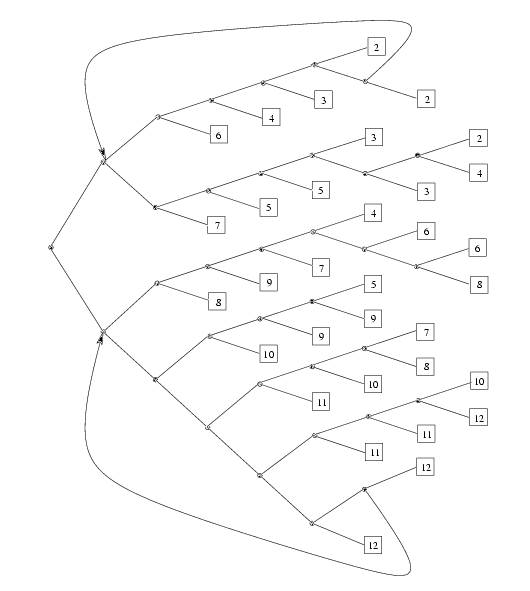
\includegraphics[scale=0.4]{images/CS3.png}
    \caption{States and transitions of the two dice model, taken from \cite{PRISMDICE}}
    \label{fig:ce3}
\end{figure}
Each one of the nodes in Figure \ref{fig:ce3}, represents a state in the probabilistic Event-B model. Therefore, the new context is going to specify a deffered set with 33 states, and an extra 34th state to specify a terminating state.
\begin{maude}

CONTEXT ctxDiceProgram2
SETS 
    STATES : { s0, s1, ... , s33, s34 }
CONSTANTS 
END
\end{maude}
For the variables, and the initialization of the machine, the Event-B specification is identical. Finally, for the events the principle is the same: For each one the transitions use a probabilistic assignment to symbolize the fifty-fifty chance in the system transitions. The resulting probabilistic Event-B model and the encoded version in PMaude, can be consulted in the \texttt{DiceProgram2.b} and \texttt{DiceProgram2.maude} files respectively. The equations that define the user observations are also defined in the same manner:
\begin{maude}

eq val("obs1", {Conf < MNAME : Machine | 
                     variables: ('st |-> st , 'diceSum |-> diceSum) >} 
                     {gt | SL}  ) = toFloat(((diceSum) =b (val(elt(2))))) .
\end{maude}
In this case \texttt{"obs1"} references the case where $k = 2$, \texttt{"obs2"} references the case $k = 3$, and so on until \texttt{"obs11"}. The MultiQuaTEx formula used to verify the model is also very similar to the previous one:
\begin{maude2}

PDice2(n) = if ((s.rval("isMax") == 1.0) || (s.rval("deadlock") == 1.0)) 
            then s.rval(n) else # PDice2(n) fi ;

eval E[ PDice2("obs1") ] ;
eval E[ PDice2("obs2") ] ;
eval E[ PDice2("obs3") ] ;
eval E[ PDice2("obs4") ] ;
eval E[ PDice2("obs5") ] ;
eval E[ PDice2("obs6") ] ;
eval E[ PDice2("obs7") ] ;
eval E[ PDice2("obs8") ] ;
eval E[ PDice2("obs9") ] ;
eval E[ PDice2("obs10") ] ;
eval E[ PDice2("obs11") ] ;
\end{maude2}
Using this formula, and the parameters $\alpha = 0.01, \delta = 0.01$ and $bs = 100$, the results of the simulation using MultiVeStA where:

\begin{table}[H]
\centering
\begin{tabular}{|l|l|l|l|}
\hline
Property      & ObtainedValue      & Variance           & CI                  \\ \hline
PDice2(obs1)  & 0.03               & 0.0291037312475958 & 0.00995116917577923 \\ \hline
PDice2(obs2)  & 0.0510077519379845 & 0.0484097138712153 & 0.00997972279089514 \\ \hline
PDice2(obs3)  & 0.0853365384615385 & 0.0780579664517895 & 0.00997985024064457 \\ \hline
PDice2(obs4)  & 0.114200743494424  & 0.101162694374703  & 0.00999035979240436 \\ \hline
PDice2(obs5)  & 0.138710691823899  & 0.119473792835145  & 0.00998550057004364 \\ \hline
PDice2(obs6)  & 0.164328767123288  & 0.137328585846037  & 0.00999266014168248 \\ \hline
PDice2(obs7)  & 0.135176848874598  & 0.116907827497064  & 0.00998823325270086 \\ \hline
PDice2(obs8)  & 0.110306513409962  & 0.0981427467677965 & 0.0099897800415653  \\ \hline
PDice2(obs9)  & 0.0811616161616162 & 0.0745781747981354 & 0.00999816628115168 \\ \hline
PDice2(obs10) & 0.0551798561151079 & 0.0521387905863524 & 0.00997746359029961 \\ \hline
PDice2(obs11) & 0.0282191780821918 & 0.0274266131408506 & 0.0099855441351178  \\ \hline
\end{tabular}
\end{table}

\begin{figure}[H]
    \centering
    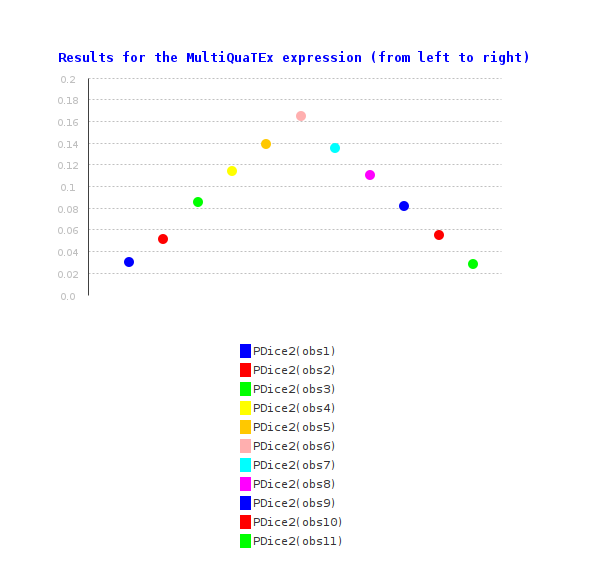
\includegraphics[scale = 0.5]{images/CS4.png}
    \caption{Graph of the simulation results of the second dice program}
    \label{fig:ce4}
\end{figure}

In total, the time it took to complete the simulation was 4583.059 seconds (76 minutes), and the results of the simulation are very close to the expected probability for each one of the possible values of the sum of the 2 dice.




    